\subsection{Blockschaltbild}
\label{subsec:Blockschaldbild}

Das im Projekt 5 entstandene Blockschaltbild ist nun um weitere Teilsysteme ergänzt worden, gemäss Abbildung \ref{fig:Blockschaltbild_Partymixer}, auf welche mit den vorherigen Teilsystemen im folgenden Kapitel\ref{sec:Printaufbau} und \ref{sec:Teilsysteme} eingegangen wird. Zu den neuen Systemen gehört ein Bluetooth- / Wirelessmodul, welches eine externe Ansteuerung per Web-Server oder Android App ermöglicht, eine dazugehörige Programmierschnittstelle, ein RFID Lesegerät, ein SD-Karten Slot und eine Maschinenbeleuchtung.

\begin{figure}[h!]
\center
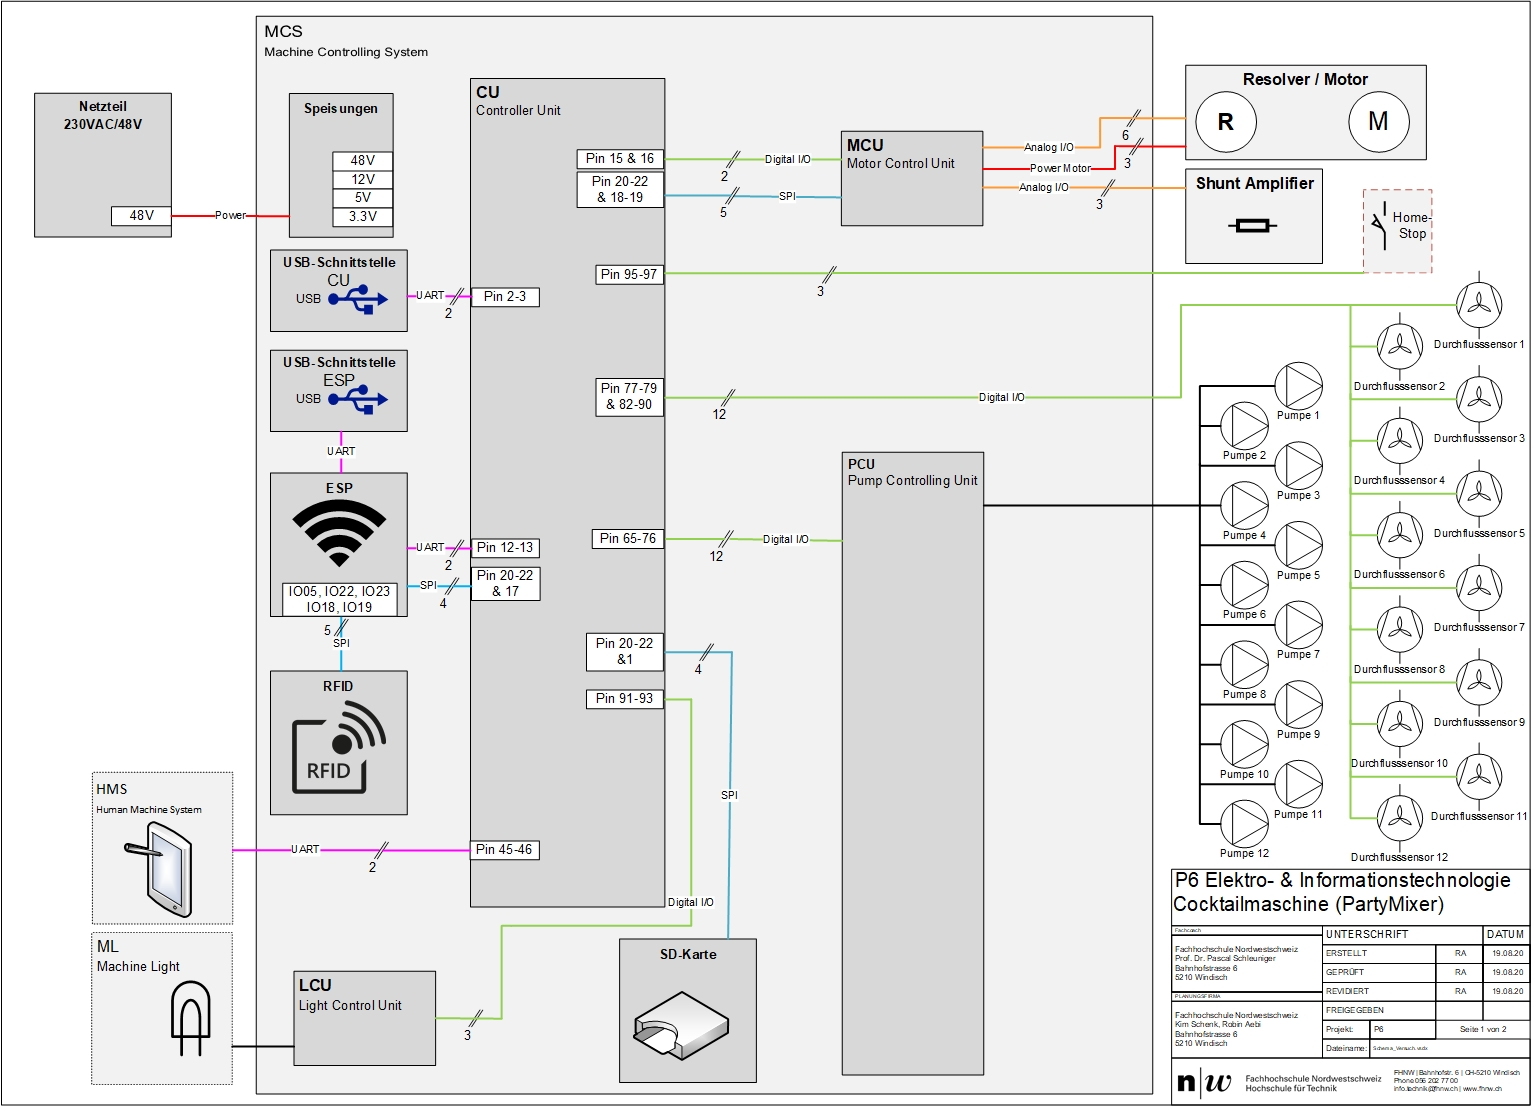
\includegraphics[angle=90, width = 0.85\textwidth]{graphics/Blockschaltbild}
\caption{Blockschaltbild des PartyMixer's gemäss Projekt 6.}
\label{fig:Blockschaltbild_Partymixer}
\end{figure}

\todo{Blockschaltbild Leitungen des Motors anpassen!}
\todo{Beide Blockschaltbilder in eins bringen und Unterschiede P5/P6 hervorheben.}

\newpage

